%!TEX root = index.tex

\section{Solving the cubic}
\begin{figure}[H]
	\begin{flushright}
	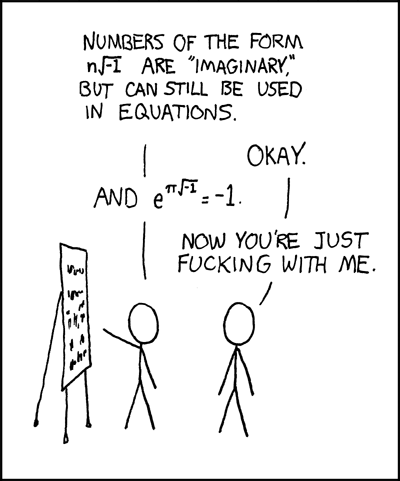
\includegraphics[width=0.6\linewidth]{resources/179.png}
	\caption*{\href{https://xkcd.com/179/}{\tiny {xkcd.com/179}}}
\end{flushright}
\end{figure}	

There is no unique way to find the roots of the cubic. We'll choose the method that is motivated by Galois theory. It'll look extremely mysterious but this is the method that generalizes to show that there is no formula for solving a general fifth degree polynomial.\\

The fundamental theorem of algebra guarantees the existence of \emph{real or complex roots} to any polynomial, as such complex numbers naturally show up when studying polynomials. 

\begin{questions}
	\item 
	\begin{enumerate}
		\item Find the three roots of the polynomial $ x^3 - 1$.
		\item Show that if one complex root of this equation is $ \omega $ then the other complex root is $ \omega^2$. Conclude that $ \conj{\omega} = \omega^2$.
    \item Compute $ \omega + \omega^2$.
		\item Plot $ \omega$, $\omega^2$ on the complex plane.
	\end{enumerate}
  $ \omega$ and $ \omega^2$ (and also 1) are called the \textbf{third roots of unity} as they satisfy $ x^3 = 1$.
\end{questions}


\begin{questions}[resume]
  \item What are the \emph{second} and the \emph{fourth} roots of unity? Plot them on the complex plane.
\end{questions}






\newpage
\subsection{The Solution}
  The method for solving the cubic is somewhat like induction, we reduce the problem to a lower degree one. We need to find intermediate constants $ \mu_1$ and $ \mu_2$ which satisfy a known \emph{quadratic} and from which $ \beta_1, \beta_2, \beta_3$ can be easily recovered.

  \textbf{Define}
  \begin{align}
    \label{eq:eq1}
    \mu_1 &= \beta_1 + \beta_2 \omega + \beta_3 \omega^2 \\
    \label{eq:eq2}
    \mu_2 &= \beta_1 + \beta_2 \omega^2 + \beta_3 \omega
  \end{align}
Recall that we also have a third equation 
\begin{align}
  \label{eq:eq3}
  0 = \beta_1 + \beta_2 + \beta_3
\end{align}

\begin{questions}[resume]
  \item Determine $ \mu_1 .\mu_2$ in terms of $p, q$.
\end{questions}

\begin{questions}[resume]
  \item 
  \begin{enumerate}
    \item Verify that the following solves the equations \eqref{eq:eq1}, \eqref{eq:eq2}, and \eqref{eq:eq3} 
      \begin{align*}
        \beta_1 = \dfrac{\mu_1 + \mu_2}{3} 
        \mbox { , } \beta_2 = \dfrac{\omega^2 \mu_1 + \omega \mu_2}{3}
        \mbox { , } \beta_3 = \dfrac{\omega \mu_1 + \omega^2 \mu_2}{3}
      \end{align*}
    Note that we have three simultaneous (non-degenerate) equations and three variables so there is a unique solution.
    \item Compute $ \beta_1 . \beta_2 . \beta_3$ in terms of $ \mu_1, \mu_2$.
    \item Use this to compute $ \mu_1^3 + \mu_2^3$ in terms of $p, q$.
  \end{enumerate}
\end{questions}


\begin{questions}[resume]
\item Find the coefficients of the quadratic polynomial whose roots are $\mu_1^3, \mu_2^3$ and hence find $ \mu_1^3$ and $ \mu_2^3$ in terms of $ p,q$.
\end{questions}


\newpage

Assuming you did the computations in the previous problems correctly, you should now have the following method for finding the roots of the cubic $P(x) = x^3 + px + q$,
  \begin{itemize}
    \item Solve the quadratic $$x^2 + 27q .x - 27 p^3 = 0$$ and pick $ \mu_1^3$ to be any one of the two roots and hence find $ \mu_1$.\footnote{Just as (unless $ a=0$) the equation $ x^2=a^2 $ has 2 solutions $ \pm a$ the equation $ x^3=a^3 $ has 3 solutions $ a, a \omega, a \omega^2$. 
    Hence we need to \emph{choose} a value of $ \mu_1$ once we know what $ \mu_1^3$ is. 
    The choice does not matter as choosing a different cube root simply permutes the roots. But the same is true for $ \mu_2$ and suddenly we have 9 choices instead of 3, hence we use the equation $ \mu_1 \mu_2 = -3p$ to determine $ \mu_2$.}
    \item Find $ \mu_2$ using $$ \mu_1 \mu_2 = -3p$$
    \item The three roots are given by
      \begin{align*}
        \beta_1 = \dfrac{\mu_1 + \mu_2}{3} 
        \mbox { , } \beta_2 = \dfrac{\omega^2 \mu_1 + \omega \mu_2}{3}
        \mbox { , } \beta_3 = \dfrac{\omega \mu_1 + \omega^2 \mu_2}{3}
      \end{align*}
  \end{itemize}
If the cubic is not depressed then we first need to shift the roots to get rid of the $ x^2$ coefficient.\\\\


\iffalse To fix this notice that by the first part of the previous problem $ \mu_1 \mu_2$ is completely determined by $ p$ and $ q$ hence once we find $ \mu_1$ we automatically get $ \mu_2$. We're now left with 3 choices for $ \mu_1$. It turns out that these three choices merely change the order of the roots $ \beta_1, \beta_2, \beta_3$ and hence any choice is equally good. 
\fi

\begin{questions}[resume]
  \item Use the above method to find the roots of 
    \begin{enumerate}
      \item $ x^3 - 1$
      \item $ x^3 + 1$
      \item $ x^3 - 3x + 2$
      \item $ x^3 - x$
    \end{enumerate} 
\end{questions}

\newpage
\subsection{Symmetries \& the Cubic }
What just happened?\\

The secret reason why the above method worked is that $ \mu_1^3$, $\mu_2^3$ remain unchanged when we cyclically permute the three roots, but not when we swap just two of them. 
\begin{questions}[resume]
  \item 
  \begin{enumerate}
    \item Compute $ \omega \mu_1$ and $ \omega^2 \mu_1$, similarly for $ \mu_2$.
    \item Use these to show that if we cyclically permute $ \beta_1, \beta_2, \beta_3$ then $ \mu_1^3$  and $ \mu_2^3$ remain unchanged.
    \item Verify that if we swap $ \beta_2$ and $ \beta_3$ then $ \mu_1^3$ and $ \mu_2^3$ also get swapped. 
    \item (optional) Show that if we swap $ \beta_1$ and $ \beta_2$ (or $ \beta_1$ and $ \beta_3$) then $ \mu_1^3$ and $ \mu_2^3$ also get swapped. 
    \item Argue that $ \mu_1^3 + \mu_2^3$ and $ \mu_1^3.\mu_2^3$ are symmetric in $ \beta_1, \beta_2, \beta_3$ (but not $\mu_1^3,\mu_2^3$ individually), and hence they are the roots of a quadratic whose coefficients are polynomials in $ p,q$.\footnote{These statements are false for $ \mu_1$ and $ \mu_2$ (instead of $ \mu_1^3$ and $ \mu_2^3$) and so there is no quadratic, with coefficients polynomials in $ p,q$, whose roots are $ \mu_1, \mu_2$. }
  \end{enumerate}
\end{questions}

Galois' work then proves that this is the only method that can give us a \emph{general} formula involving radicals. He then went on to show that no such intermediate variables exist for a fifth degree polynomial. \\

\noindent There is another pair which we've already encountered that also has these symmetries. 
\begin{align*}
  \sqrt{\Delta} &= (\beta_1 - \beta_2)(\beta_2 - \beta_3)(\beta_3 - \beta_1) 
  \\
  -\sqrt{\Delta} &= (\beta_2 - \beta_1)(\beta_3 - \beta_2)(\beta_1 - \beta_3)
\end{align*}
\begin{questions}[resume]
    \item Verify that both $\sqrt{\Delta}$ and $-\sqrt{\Delta}$ remain unchanged under cyclic permutation of roots and get swapped when we swap two of the $ \beta_i$'s.
\end{questions}
This isn't a coincidence, you can rewrite the solutions you found in terms of $ \pm \sqrt {\Delta}$. In fact \emph{any} variables with these symmetries should provide us with a solution to the cubic, which variables we use is a matter of convenience.

\begin{questions}[resume]
    \item Go back to your formulae for $ \mu_1^3$ and $ \mu_2^3$ and express them them terms of $ p, q$ and $ {\Delta}$.
\end{questions}






\iffalse
\subsection{Optional questions}
It is a very difficult question in general to determine whether a polynomial with integer coefficients can be written as a product of two polynomials with integer coefficients of smaller degrees. But in the case of $ p(x) = x^n - 1$ we know the answer to this question. The irreducible factors of $ x^n - 1$ are called \textbf{cyclotomic polynomials} and there is \emph{exactly one} of each degree.

	\begin{questions}[resume]
	  \item Define the $ n^{th}$ cyclotomic polynomial as
			\begin{align*}
				\Phi_n(x) = \prod (x - e^{2 \pi i k/n})
			\end{align*}
			where the product is taken over all $ 1 \le k \le n $ such that $ \gcd(k,n) = 1$.
			\begin{enumerate}
				\item Compute $ \Phi_2(x)$, $ \Phi_3(x)$, $ \Phi_4(x)$.
				\item Compute $ \Phi_p(x)$ when $ p$ is a prime.
				\item Show that $ \Phi_n(x)$ divides the polynomial $x^n - 1$.
				\item In fact show that
					\begin{align*}
						x^n - 1 = \prod \limits_{d|n} \Phi_d(x)
					\end{align*}
			\end{enumerate}
			It is a non-trivial fact that the coefficients of $ \Phi_n(x)$ are all integers. It is an ever more non-trivial fact that the cyclotomic polynomials $ \Phi_n(x)$ are all irreducible. One way to prove these facts is using Galois theory.
	\end{questions}
\fi